\documentclass[10pt]{beamer}

\usetheme{metropolis}
\usepackage{appendixnumberbeamer}

\usepackage{booktabs}
\usepackage[scale=2]{ccicons}
\usepackage{graphicx}
\usepackage{hyperref}
\usepackage{circuitikz}
\usepackage{pdflscape}
\usepackage{smartdiagram}

\usepackage{color}
\usepackage{listings}

\lstset{
	basicstyle=\footnotesize\ttfamily,
    keepspaces=true,
    showstringspaces=false,
    language=PHP,
    commentstyle=\ttfamily,
}

\usepackage[OT4]{polski}
\usepackage[utf8]{inputenc}

\usepackage{pgfplots}
\usepgfplotslibrary{dateplot}

\usepackage{xspace}
\newcommand{\themename}{\textbf{\textsc{metropolis}}\xspace}

\setbeamertemplate{frame footer}{}
\setbeamertemplate{frame numbering}{}

\usetikzlibrary{shapes,arrows}

\tikzstyle{decision} = [diamond, draw, fill=blue!20, 
    text width=4.5em, text badly centered, node distance=3cm, inner sep=0pt]
\tikzstyle{block} = [rectangle, draw, fill=blue!20, 
    text width=5em, text centered, rounded corners, minimum height=4em]
\tikzstyle{line} = [draw, -latex']
\tikzstyle{cloud} = [draw, ellipse,fill=red!20, node distance=3cm,
    minimum height=2em]


\title{Obsługa zapytań, protokół HTTP}

\subtitle{Zaawansowane metody programowania}
\author{mgr inż. Krzysztof Rewak}
\date{\today}
\institute{Wydział Nauk Technicznych i Ekonomicznych \\ Państwowa Wyższa Szkoła Zawodowa im. Witelona w Legnicy}

\begin{document}

\maketitle

\begin{frame}{Plan prezentacji}
  \setbeamertemplate{section in toc}[sections numbered]
  \tableofcontents[hideallsubsections]
\end{frame}


\section{Serwery dla systemów internetowych}

\begin{frame}{Serwer? Jaki serwer?}
	Jak uruchomić system internetowy napisany w dowolnym języku?
\end{frame}

\begin{frame}[fragile]{Budowa klasycznego systemu internetowego}
	\begin{tikzpicture}[node distance=3cm, minimum size=2cm, auto]
	
		\node [block] (core) {jądro systemu};
	
		\node [block, above of=core] (server) {funkcje serwerowe};
		\node [block, left of=core] (database) {bazy danych};
		\node [block,above left of=core] (cache) {serwery cache};
		\node [block, below left of=core] (filesystem) {systemy plików};
		\node [block, below of=core] (services) {inne serwisy};
	
		\path [line] (core) -- node {} (server);
		\path [line] (server) -- node {} (core);
	
		\path [line] (core) -- node {} (database);
		\path [line] (database) -- node {} (core);
	
		\path [line] (core) -- node {} (cache);
		\path [line] (cache) -- node {} (core);
	
		\path [line] (core) -- node {} (filesystem);
		\path [line] (filesystem) -- node {} (core);
	
		\path [line] (core) -- node {} (services);
		\path [line] (services) -- node {} (core);
		
		\node [circle, fill=orange,inner sep=3pt, right of=core] (http) {serwer HTTP};
	
		\path [line] (http) -- node {} (core);
		\path [line] (core) -- node {} (http);
		
		\node [block, above right of=http] (browser) {przeglądarka};
		\node [block, below right of=http] (api) {inna aplikacja};
	
		\path [line] (http) -- node {} (browser);
		\path [line] (browser) -- node {} (http);
	
		\path [line] (http) -- node {} (api);
		\path [line] (api) -- node {} (http);
	\end{tikzpicture}
\end{frame}

\begin{frame}{Obsługa zapytań}
	Co się dzieje po wpisaniu w pasek adresu przeglądarki internetowej adresu \texttt{http://pwsz.rewak.pl}?
\end{frame}

\begin{frame}{Obsługa zapytań}
	\begin{figure}[t]
		\centering
		\includegraphics[width=\linewidth]{addressbar.png}
		\caption{Adres wpisany do paska adresu}
	\end{figure}
\end{frame}

\begin{frame}[fragile]{Uproszczony cykl życia zapytania}
	\hspace*{-1cm}%
	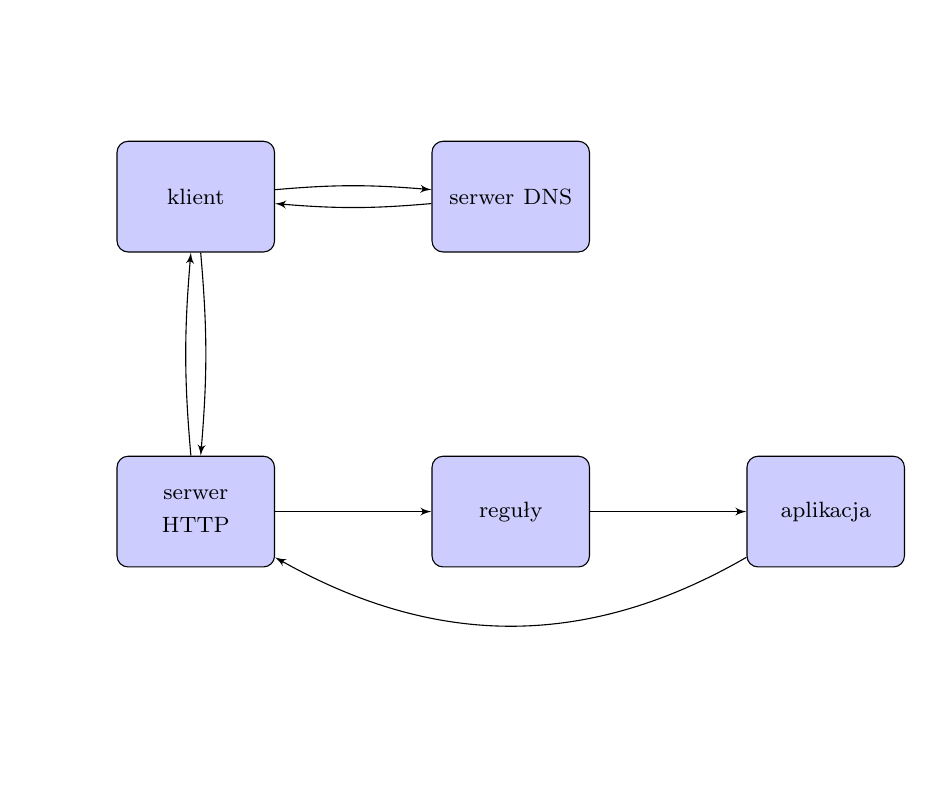
\begin{tikzpicture}[node distance=4cm, minimum size=2cm, auto]
		\node [block] (request) {\footnotesize klient};
		\node [block, right of=request] (dns) {\footnotesize serwer DNS};
		\node [block, below of=request] (http) {\footnotesize serwer HTTP};
		\node [block, right of=http] (rules) {\footnotesize reguły};
		\node [block, right of=rules] (app) {\footnotesize aplikacja};
		
		\path [line] (request) edge [bend left=5] node {} (dns);
		\path [line] (dns) edge [bend left=5] node {} (request);
		\path [line] (request) edge [bend left=5] node {} (http);
		\path [line] (http) edge node {} (rules);
		\path [line] (rules) edge node {} (app);
		\path [line] (app) edge [bend left=30] node {} (http);
		\path [line] (http) edge [bend left=5] node {} (request);
	\end{tikzpicture}
\end{frame}

\begin{frame}{Funkcje serwera HTTP}
	Czego powinniśmy wymagać od serwera HTTP:
	\begin{itemize}
		\item obsługi przychodzących zapytań (najczęściej nasłuchując portu :80)
		\item wyświetlania plików z wyznaczonych katalogów
		\item możliwości uruchomienia innych serwisów
	\end{itemize}
	
	Każdy z popularnych serwerów oczywiście dostarcza wielu innych ciekawych rozwiązań.
\end{frame}

\begin{frame}[fragile]{Przykład \emph{uno}}
	Po wpisaniu adresu
	\begin{lstlisting}
www.pwsz.legnica.edu.pl/test.html
	\end{lstlisting}
	
	przeglądarka wyśle zapytanie
	\begin{lstlisting}
GET /test.html HTTP/1.1
Host: www.pwsz.legnica.edu.pl
	\end{lstlisting}
	
	na adres IP 156.17.194.34; serwer Apache obsługujący serwer najpewniej przekierowuje cały ruch na konkretny katalog, na przykład
	\begin{lstlisting}
/home/www/pwsz-web/
	\end{lstlisting}
	
	Serwer zwraca błąd 404 (\emph{The requested URL /test.html was not found on this server}) i pokazuje szereg ciekawych informacji o serwerze: \texttt{Apache/2.2.9 (Debian) PHP/5.2.6-1+lenny16 with Suhosin-Patch mod\_ssl/2.2.9 OpenSSL/0.9.8g Server at www.pwsz.legnica.edu.pl Port 80}
\end{frame}

\begin{frame}[fragile]{Przykład \emph{dos}}
	Po wpisaniu adresu
	\begin{lstlisting}
www.pwsz.rewak.pl/test.html
	\end{lstlisting}
	
	przeglądarka wyśle zapytanie
	\begin{lstlisting}
GET /test.html HTTP/1.1
Host: www.pwsz.rewak.pl
	\end{lstlisting}
	
	na adres IP 85.255.1.83; serwer Apache obsługujący mój serwer łapie prawie cały ruch z tej domeny i przekierowuje go na plik
	\begin{lstlisting}
/home/www/pwsz.rewak.pl/public/index.html
	\end{lstlisting}
	
	Tam załaduje się frontendowa aplikacja, która zbada URL i zwróci odpowiedź, że taki plik nie istnieje.
\end{frame}

\begin{frame}[fragile]{Przykład \emph{tré}}
	Po wpisaniu adresu
	\begin{lstlisting}
www.pwsz.rewak.pl/api/courses
	\end{lstlisting}
	
	przeglądarka wyśle zapytanie
	\begin{lstlisting}
GET /api/courses HTTP/1.1
Host: www.pwsz.rewak.pl
	\end{lstlisting}
	
	na adres IP 85.255.1.83; serwer Apache obsługujący mój serwer złapie zapytanie do nibykatalogu \texttt{api} i przekieruje resztę zapytania do pliku
	\begin{lstlisting}
/home/www/pwsz.rewak.pl/public/index.php
	\end{lstlisting}
	
	Przeglądarka otrzyma JSON-a z listą wszystkich prowadzonych przez mnie kursów.
\end{frame}

\begin{frame}{Najpopularniejsze rozwiązania}
	\begin{itemize}
		\item Apache: 47\%
		\item Nginx - 37\%
		\item IIS - 10\%
		\item LiteSpeed - 3\%
		\item Google - 1\%
		\item pozostałe: Tomcat, Node.js, ATS, IWS...
	\end{itemize}
\end{frame}

\begin{frame}[fragile]{Magia plików \texttt{.htaccess}}
	Plik umieszczony w katalogu projektu może nadpisać ustawienia Apache. Przykładowo można przekierować cały przekierowany ruch na inny katalog:
	\begin{lstlisting}
<IfModule mod_rewrite.c>
	RewriteEngine on
	RewriteRule  ^$ public/    [L]
	RewriteRule  (.*) public/$1 [L]
</IfModule>
	\end{lstlisting}
	
	Warto zapamiętać, że dobrą praktyką jest przekierowanie zapytań HTTP na publiczny folder, w którym nie będzie dostępnych plików aplikacji, repozytorium, itp.
\end{frame}

\begin{frame}[fragile]{Magia plików \texttt{.htaccess}}
	Można również przykładowo zablokować dostęp do katalogu wszystkim, którzy nie podadzą poprawnego hasła:
	\begin{lstlisting}
AuthType Basic
AuthName "Password Protected Area"
AuthUserFile /path/to/.htpasswd
Require valid-user
	\end{lstlisting}
\end{frame}

\begin{frame}[fragile]{Magia plików \texttt{.htaccess}}
	Pliki \texttt{.htaccess} pozwolą również na:
	
	\begin{itemize}
		\item zarządzanie listowaniem zawartości katalogów,
		\item własne strony błędów,
		\item obsługę typów plików,
		\item zarządzanie pamięcią podręczną.
	\end{itemize}
	
	 Zmiany są natychmiastowe (ponieważ plik jest wczytywany przy każdym zapytaniu), ale spowalniają serwer.
\end{frame}

\begin{frame}{Porównanie funkcjonalności serwerów webowych}
	\begin{figure}[t]
		\centering
		\includegraphics[width=\linewidth]{table.png}
		\caption{Tabela porównawcza wg \url{https://en.wikipedia.org/wiki/Comparison_of_web_server_software}}
	\end{figure}
\end{frame}

\section{HTTP i jego metody}

\begin{frame}{Metody zapytań}
	Specyfikacja protokółu HTTP/1.0 wyróżnia kilka podstawowych metod komunikacji z serwerem. Wystosowane z poziomu klienta zapytanie ma w nagłówku informację na temat wybranej metody, a wyróżniamy m. in.:
	
	\begin{itemize}
		\item \texttt{GET}
		\item \texttt{POST}
		\item \texttt{PUT}
		\item \texttt{DELETE}
		\item \texttt{OPTIONS}
		\item i inne
	\end{itemize}
\end{frame}

\begin{frame}[fragile]{Metoda \texttt{GET}}
	Podstawowa metoda przeznaczona \textbf{tylko i wyłącznie} do pobierania danych.
	
	Lista parametrów przekazanych w zapytaniu dodawana jest do URL-a:
	\begin{lstlisting}
http://example.com/index.php?query=Test&country_iso=pl
	\end{lstlisting}
\end{frame}

\begin{frame}[fragile]{Metoda \texttt{POST}}
	Podstawowa metoda przeznaczona do przesyłania danych, które mają wpłynąć na system. Serwer oczywiście zwróci odpowiedź w identyczny sposób jak przy metodzie \texttt{GET}.
	
	Przykładowo \texttt{POST}-em należy wysyłać dane z formularzy czy żądania zmiany statusu. 
\end{frame}

\begin{frame}[fragile]{RESTful API i etody \texttt{PUT},  \texttt{PATCH} i \texttt{DELETE}}
	Sprytnie zaprojektowana aplikacja rozróżnia wywołania tego samego URL-a z różnymi metodami. REST-owe API może działać następująco:
	
	\begin{itemize}
		\item \texttt{GET /users} zwróci listę użytkowników
		\item \texttt{PUT /users} podmieni listę użytkowników przesłaną nową listą
		\item \texttt{POST /users} doda nowego użytkownika
		\item \texttt{DELETE /users} usunie listę użytkowników
	\end{itemize}
	
	\begin{itemize}
		\item \texttt{GET /users/1} zwróci użytkownika o danym \texttt{id = 1}
		\item \texttt{PUT /users/1} podmieni użytkownika lub go utworzy
		\item \texttt{PATCH /users/1} podmieni użytkownika
		\item \texttt{DELETE /users/1} usunie użytkownika
	\end{itemize}
	
\end{frame}

\section{Zapytanie i odpowiedź}

\begin{frame}[fragile]{Zapytanie}
	Zapytanie (\emph{Request}) wysyłane przez przeglądarkę oczywiście nie składa się tylko z hosta:

	\begin{lstlisting}
GET / HTTP/1.1
Host: pwsz.rewak.pl
User-Agent: Mozilla/5.0 (Windows NT 10.0; Win64; x64; rv:58.0)
	Gecko/20100101 Firefox/58.0
Accept: text/html,application/xhtml+xml,
	application/xml;q=0.9,*/*;q=0.8
Accept-Language: pl,en-US;q=0.7,en;q=0.3
Accept-Encoding: gzip, deflate
Cookie: _ga=GA1.2.251979732.1506974412; 
	_gid=GA1.2.724276722.1520606158
Connection: keep-alive
Upgrade-Insecure-Requests: 1
	\end{lstlisting}
\end{frame}

\begin{frame}[fragile]{Odpowiedź}
	Natomiast odpowiedź zawsze zawiera w sobie nagłówek (\emph{Response header}) oraz zawartość (\emph{Response body}). Nagłówek wygląda zazwyczaj jak poniżej:

	\begin{lstlisting}
Accept-Ranges: bytes
Connection: Keep-Alive
Content-Encoding: gzip
Content-Length: 432
Content-Type: text/html; charset=UTF-8
Date: Sun, 11 Mar 2018 10:02:19 GMT
ETag: "2a4-55b3fcc244d5e-gzip"
Keep-Alive: timeout=5, max=100
Last-Modified: Wed, 11 Oct 2017 06:47:29 GMT
Server: Apache/2.4.18 (Ubuntu)
Vary: Accept-Encoding
	\end{lstlisting}
\end{frame}

\begin{frame}[fragile]{Odpowiedź}
	Zawartość to oczywiście HTML strony internetowej:

	\begin{lstlisting}
<!DOCTYPE html>
<html>
<head>
   <meta charset="utf-8">
   <meta http-equiv="X-UA-Compatible" content="IE=edge">
   <meta name="viewport"
     content="width=device-width,initial-scale=1">
   <title>Krzysztof Rewak</title>
   <link rel="stylesheet"
     href="/static/css/app.c0927d6b397cd98ad145970e94ff4c51.css">
</head>

(...)
	\end{lstlisting}
\end{frame}

\section{Kody statusów}

\begin{frame}{Kody statusów}
	Każda odpowiedź serwera ma przypisany do siebie specjalny kod statusu, który powinien powiedzieć przeglądarce i użytkownikowi, co stało się z jego zapytaniem.
	
	
	Kody są pogrupowane według typu odpowiedzi i można je szybko zidentyfikować po pierwszej cyfrze trzycyfrowego kodu.
\end{frame}

\begin{frame}{Kody statusów}
	\begin{figure}[t]
		\centering
		\includegraphics[width=\linewidth]{responses.png}
		\caption{Narzędzia deweloperskie mocno pomagają przy badaniu komunikacji z serwerem}
	\end{figure}
\end{frame}

\begin{frame}{Przykładowe kody statusów}	
	\begin{itemize}
		\item \textbf{1xx} informacje zwrotne
		\item \textbf{2xx} informacje o sukcesie:
		\begin{itemize}
			\item \textbf{200} OK
			\item \textbf{201} Created
			\item \textbf{202} Accepted
		\end{itemize}
		\item \textbf{3xx} informacje o przekierowaniu
		\item \textbf{4xx} informacje o błędzie po stronie klienta:
		\begin{itemize}
			\item \textbf{400} Bad Request
			\item \textbf{401} Unauthorized
			\item \textbf{403} Forbidden
			\item \textbf{404} Not Found
			\item \textbf{405} Method Not Allowed
		\end{itemize}
		\item \textbf{5xx} informacje o błędzie po stronie serwera:
		\begin{itemize}
			\item \textbf{500} Internal Server Error
			\item \textbf{501} Not Implemented
			\item \textbf{503} Service Unavailable
			\item \textbf{504} Gateway Timeout
		\end{itemize}
	\end{itemize}
\end{frame}

\section{Routing}

\begin{frame}{Najprostsza aplikacja w PHP}
	Najprymitywniejsza aplikacja napisana w PHP mogłaby mieć taką strukturę:

	\begin{itemize}
		\item \texttt{styles/}
		\begin{itemize}
			\item \texttt{style.css}
		\end{itemize}
		\item \texttt{dashboard.php}
		\item \texttt{index.php}
		\item \texttt{login.php}
		\item \texttt{logout.php}
		\item \texttt{register.php}
	\end{itemize}
	
	Jeżeli Apache lub Nginx wskazuje folder projektu, wówczas wystarczy w pasku adresu wpisać \texttt{localhost/login.php}, aby otworzyć stronę do logowania.
\end{frame}

\begin{frame}{Najprostsza aplikacja w PHP}
	Jest to pomysł przynajmniej beznadziejny.
\end{frame}

\begin{frame}{Router systemów internetowych}
	Router jest częścią aplikacji, która odpowiada za przypisanie konkretnych akcji do wywoływanych adresów URL.
	
	Najczęstsza konfiguracja to wskazanie serwerowi, aby zawsze przekierowywał domenę na jeden plik (\texttt{index.php}) lub serwis (WSGI). Wówczas już aplikacja zajmie się rozprowadzaniem zadań, a nie serwer HTTP.
\end{frame}

\begin{frame}[fragile]{Router w Django}
	\begin{lstlisting}
from django.urls import path
from app import views

urlpatterns = [
    path('/', views.get_index),
    path('/faq', views.get_faq),
    path('/about', views.get_about),
    path('/login', views.get_login),
    path('/user/<ind:id>', views.get_user_page),
]
	\end{lstlisting}
\end{frame}

\begin{frame}[fragile]{Router w Laravelu}
	\begin{lstlisting}
<?php

Route::get('/', 'HomeController@getIndex');
Route::get('/faq', 'HomeController@geFaq');
Route::get('/about', 'HomeController@getAbout');
Route::get('/login', 'LoginController@get');
Route::post('/login', 'LoginController@post');
Route::get('/user/:id', 'UserController@getUserPage');
	\end{lstlisting}
\end{frame}

\begin{frame}[fragile]{Router w ASP.NET MVC}
	\begin{lstlisting}
public class HomeController : Controller
{
	[Route('/')]
	public ActionResult View()
	{
		return View('Home');
	}
	
	[Route('about')]
	public ActionResult View()
	{
		return View('About');
	}
}
	\end{lstlisting}
\end{frame}

\section{Podsumowanie}

\begin{frame}{Bibliografia i ciekawe źródła}
  
	\begin{thebibliography}{9}
	
		\bibitem{w3}
		\url{https://w3techs.com/technologies/overview/web_server/all}
		
		\bibitem{http}
		\url{https://en.wikipedia.org/wiki/Hypertext_Transfer_Protocol}
		
		\bibitem{codes}
		\url{https://en.wikipedia.org/wiki/List_of_HTTP_status_codes}
		
		\bibitem{headers}
		\url{https://en.wikipedia.org/wiki/List_of_HTTP_header_fields}
	
	\end{thebibliography}

\end{frame}

\appendix

\begin{frame}[standout]
	Pytania?
\end{frame}

\begin{frame}{}

	Kod prezentacji dostępny jest w repozytorium git pod adresem \texttt{https://bitbucket.org/krewak/pwsz-zmp} \\ \ \\

	\begin{figure}
		\centering
		\href{https://bitbucket.org/krewak/pwsz-ppsi}{
			\includegraphics[width=.15\textwidth]{../_template/bitbucket.png}
		}
	\end{figure}
	
	Wszystkie informacje dot. kursu dostępne są pod adresem \texttt{http://pwsz.rewak.pl/kursy/10} \\ \ \\

	\begin{figure}
		\centering
		\href{http://pwsz.rewak.pl/kursy/3}{
			\includegraphics[width=.15\textwidth]{../_template/rewak.png}
		}
	\end{figure}

\end{frame}

\end{document}
